\documentclass{article}
\usepackage{graphicx} % Required for inserting images
\usepackage{tikz}
\usepackage{svg}
\usepackage{amsmath}

\title{Problem Set 1}
\author{Aleksandr Efremov}
\date{July 2023}

\begin{document}

\maketitle

\section{Part I}
\subsection{Recitation 0}
\begin{itemize}
\item[(1A-1a)] $y = x^2 - 2x - 1 = (x - 1)^2 - 2$
\begin{figure}[htp!]
    \centering
    \includesvg{graph-1.svg}
    \label{fig:fig1}
\end{figure}
\newpage
\item[(1A-2a)] $y = 1 + |x + 2|$
\begin{figure}[htp!]
    \centering
    \includesvg{graph-2.svg}
    \label{fig:fig2}
\end{figure}

\item[(1A-3a)] $f(x) = \frac{x^3+3x}{1-x^4}$ \\ \\
$f(x)$ is $odd$. \\ \\
$f(-x) = \frac{(-x)^3+3(-x)}{1 - (-x)^4} = \frac{-x^3-3x}{1-x^4} = -\frac{x^3+3x}{1-x^4} = -f(x)$

\item[(1A-3b)] $f(x) = \sin^2 x$ \\ \\
$f(x)$ is $even$. \\ \\
$f(-x) = \sin^2(-x) = \sin(-x)\sin(-x) = (-\sin x)(-\sin x) = \sin^2 x = f(x)$

\item[(1A-3e)] $f(x) = J_0(x^2)$ \\ \\
$f(x)$ is $even$. \\ \\
$f(-x) = J_0((-x)^2) = J_0(x^2) = f(x)$

\item[(1A-6a)] $A\sin (x + c) = A\sin x \cos c + A\cos x \sin c$ \\ \\
$A = 2$, $c = \frac{\pi}{3}$ \\ \\
$2\sin(x+\frac{\pi}{3}) = 2\sin x \cos \frac{\pi}{3} + 2\cos x \sin \frac{\pi}{3} = \sin x + \sqrt{3}\cos x$

\item[(1A-7a)] $y = 3\sin (2x - \pi)$ \\ \\
Rewrite function as $y = 3 \sin 2(x-\frac{\pi}{2})$. The period is $\pi$, amplitude is $3$ and phase angle is $\frac{\pi}{2}$.

\begin{figure}[htp!]
    \centering
    \includesvg{graph-3.svg}
    \label{fig:fig4}
\end{figure}

\end{itemize}

\subsection{Lecture 1}
\begin{itemize}
\item[(1C-3a)] $f(x) = \frac{1}{2x+1}$ \\ \\
\[ f'(x) = \lim_{\Delta x \to 0} \frac{1/(2(x+ \Delta x)+1) - 1/(2x+1)}{\Delta x}\]
\[ = \lim_{\Delta x \to 0} \frac{1/(2x+ 2\Delta x+1) - 1/(2x+1)}{\Delta x}\]
\[ = \lim_{\Delta x \to 0} \frac{2x + 1 - 2x - 2 \Delta x - 1}{(2x+ 2\Delta x+1)(2x+1)(\Delta x)}\]
\[ = \lim_{\Delta x \to 0} \frac{-2 \Delta x}{(2x+ 2\Delta x+1)(2x+1)(\Delta x)}\]
\[ = \lim_{\Delta x \to 0} \frac{-2}{(2x+ 2\Delta x+1)(2x+1)}\]
\[ = \frac{-2}{(2x+ 0 +1)(2x+1)} = \frac{-2}{(2x+1)^2}\]

\item[(1C-3b)] $f(x) = 2x^2 + 5x + 4$
\[ f'(x) = \lim_{\Delta x \to 0} \frac{2(x+\Delta x)^2 + 5(x+\Delta x) + 4 - 2x^2 - 5x - 4}{\Delta x}\]
\[ = \lim_{\Delta x \to 0} \frac{4x\Delta x + 2\Delta x^2 + 5\Delta x}{\Delta x}\]
\[ = \lim_{\Delta x \to 0} 4x + 2\Delta x + 5 = 4x + 5\]
\item[(1C-3e)] For part $(1C-3a)$ the slope can't be $0$ and $1$ as the derivative is negative. For slope $-1$:
\[ \frac{-2}{(2x+1)^2} = -1 \Rightarrow (2x+1)^2 = 2 \Rightarrow 2x+1 = \pm\sqrt{2}\]
\[ \Rightarrow x = -\frac{1}{2} \; \pm\ \frac{\sqrt{2}}
{2}\]

So for part $(1C-3a)$ the slope is $-1$ at $x = -\frac{1}{2} \; \pm\ \frac{\sqrt{2}}{2}$. \\ \\
For part $(1C-3b)$ the slope is $1$ when $4x + 5 = 1 \Rightarrow x = -1$. The slope is $-1$ when $4x + 5 = -1 \Rightarrow x = -\frac{3}{2}$. The slope is $0$ when $4x + 5 = 0 \Rightarrow x = -\frac{5}{4}$

\item[(1C-4a)] $f(x) = \frac{1}{2x+1}$, $f'(x) = \frac{-2}{(2x+1)^2}$ \\ \\ 
$f'(1) = \frac{-2}{9}$, $f(1) = \frac{1}{3}$ \\

$y - \frac{1}{3} = \frac{-2}{9}(x-1) \Rightarrow 
y = \frac{-2}{9}x + \frac{2}{9} + \frac{1}{3} \Rightarrow
y = \frac{-2x+5}{9}$

\item[(1C-4b)]
$f(x) = 2x^2+5x+4$, $f'(x) = 4x+5$ \\ \\ 
$f'(a) = 4a+5$, $f(a) = 2a^2+5a+4$ \\

$y - 2a^2-5a-4 = (4a+5)(x-a) \Rightarrow 
y = 4ax-4a^2+5x-5a+2a^2+5a+4 \Rightarrow
y = 4ax+5x-2a^2+4 \Rightarrow y = (4a+5)x-2(a^2-2)$
\item[(1C-5)]
$y = 1 + (x - 1)^2$, $y' = 2(x-1)$. \\
Let's find a tangent line through the point $a$. \\ \\
$y(a) = 1 + (a - 1)^2$, $y'(a) = 2(a - 1)$. \\ \\
The line has equation $y = y'(a)(x-a) + y(a)$. So,\\ \\
$y = 2(a-1)(x-a)+1+(a-1)^2$. \\ \\
Let's plug $x = 0$ and $y = 0$ to find points on the graph at which the tangent line goes through the origin.\\ \\
$0 = 2(a-1)(0-a)+1+(a-1)^2 = -2a^2+2a+1+a^2-2a+1 = -a^2+2 \Rightarrow 0 =-a^2+2 \Rightarrow a = \pm \sqrt{2}$
\\ \\
Plug $a$ in the equation of tangent line with $\pm \sqrt{2}$ to get the tangent lines through the origin. \\ \\
$y = 2(\sqrt{2}-1)(x-\sqrt{2})+1+(\sqrt{2}-1)^2 = (\sqrt{2}-1)2x$ \\

$y = 2(-\sqrt{2}-1)(x+\sqrt{2})+1+(-\sqrt{2}-1)^2 = (-\sqrt{2}-1)2x$

\item[(1C-6)]
Skipped
\item[(1B-2)] $s = bt - 16t^2$
\begin{itemize}
\item[a)] $v = \frac{ds}{dt} = b - 32t$
\item[b)] The maximum height when $v = 0$. So,
\[ b - 32t = 0 \]
\[ t = \frac{b}{32}\]
\item[c)] The maximum height is $s(\frac{b}{32}) = \frac{b^2}{32} - \frac{b^2}{64} = \frac{b^2}{64}$
\newpage
\item[d)] The graphs of $v$ and $s$
\begin{figure}[htp!]
    \centering
    \includesvg[width=\textwidth, height=10cm]{graph-5.svg}
    \caption{The graph of $v$ (one bounce)}
    \label{fig:fig5}
\end{figure}
\newpage
\begin{figure}[htp!]
    \centering
    \includesvg[width=\textwidth, height=10cm]{graph-4.svg}
    \label{fig:fig6}
    \caption{The graph of $s$ (one bounce)}
\end{figure}
\newpage
\item[e)] Let's take an initial velocity of the second bounce as $c$. Then $s = ct + 16t^2 \Rightarrow v = c + 32t$. So the maximum height of the second bounce is $\frac{c^2}{64}$. But we know that the maximum height of the second bounce is half of the first bounce, so $\frac{c^2}{64} = \frac{b^2}{64} \cdot \frac{1}{2} \Rightarrow c = \frac{b}{\sqrt{2}}$. That means that $v = \frac{b}{\sqrt{2} - 32t}$ and $s = \frac{b}{\sqrt{2}}t - 16t^2$.
\begin{figure}[htp!]
    \centering
    \includesvg[width=\textwidth, height=10cm]{graph-6.svg}
    \label{fig:fig7}
    \caption{The graph of $v$ (two bounces)}
\end{figure}
\newpage
\begin{figure}[htp!]
    \centering
    \includesvg[width=\textwidth, height=10cm]{graph-7.svg}
    \label{fig:fig8}
    \caption{The graph of $s$ (two bounces)}
\end{figure}

\item[f)] Let's examine the third bounce. If $d$ is initial velocity then it's maximum height is at time $t = \frac{d} {32}$ (starting from $0$) and its value is $\frac{d^2}{64}$, which is half of the second bounce $\frac{d^2}{64} = \frac{b^2}{128} \cdot \frac{1}{2} \Rightarrow d = \frac{b}{2}$. So the maximum height of third bounce is at time $t = \frac{b}{64}$ (starting from zero) and its value is $\frac{b^2}{256}$. The first bounce lasts $\frac{b}{16}$, the second bounce lasts $\frac{b}{16\sqrt{2}}$, the third lasts $\frac{b}{32}$ and so on. To get the time of the final landing of the ball we have to sum up all the times of individual landings of each bounce. This summation is geometric series as shown below.
\[ S = (\frac{b}{16} + \frac{b}{16\sqrt{2}} + \frac{b}{32} + \dots)\]
\[\frac{b}{16}\sum_{i = 0} ^\infty \left( \frac{1}{\sqrt{2}} \right)^i = \frac{b}{16} \cdot \frac{1}{1 - \frac{1}{\sqrt{2}}} \]

\end{itemize}

\item[(1C-1a)] The area of a disk is given by function $A(r) = \pi r^2$.
\[ \lim_{\Delta r \to 0} \frac{dA}{dr} = \frac{A(r+\Delta r) - A(r)}{\Delta r} = \lim_{\Delta r \to 0} \frac{\pi(r+\Delta r)^2 - \pi r^2}{\Delta r} \]
\[ = \lim_{\Delta r \to 0} \frac{\pi r^2 + 2 \pi r \Delta r + \pi \Delta r^2 - \pi r^2}{\Delta r} = \lim_{\Delta r \to 0} \left( 2 \pi r + \pi \Delta r \right) = 2\pi r  \]
\end{itemize}

\subsection{Lecture 2}

\begin{itemize}
\item[(1D-1)]
\begin{itemize}
    \item[(b)] $\lim_{x \to 2} \frac{4x}{x+1} = \frac{8}{3}$ 
    \item[(c)] $\lim_{x \to -2} \frac{4x^2}{x+2} = undefined (\pm \infty)$
    \item[(e)] $\lim_{x \to 2^-} \frac{4x^2}{2-x} = +\infty$
    \item[(f)] $\lim_{x \to \infty} \frac{4x^2}{x-2} = +\infty$
    \item[(g)] $\lim_{x \to \infty} \frac{4x^2}{x-2} - 4x = \lim_{x \to \infty} \frac{4x^2-4x^2+8x}{x-2} = \lim_{x \to \infty} \frac{8x}{x-2} = 8$  
\end{itemize}
\item[(1D-4a)] Skip
\item[(1C-2)] $\lim_{x \to a} \frac{(x-a)g(x) - (a - a)g(a)}{x-a} = g(x)$
\item[(1D-3)]
\begin{itemize}
    \item[(a)] $f(x) = \frac{x-2}{x^2-4}$. The point of discontinuity is $2$ since $f(2)$ is undefined. The type of discontinuity is Removable Discontinuity since $\lim_{x \to 2} f(x) = \frac{1}{4}$.
    \item[(d)] 
    \[f(x)=
    \left\{
      \begin{array}{ll}
      x+a, & x > 0 \\
      a-x, & x < 0 \\
      \end{array} 
      \right.
    \]
    The point of discontinuity is $0$ since $f(x)$ is undefined at $x = 0$. The type of discontinuity is Removable Discontinuity. 
    \item[(e)]
    \[f(x)=
    \left\{
      \begin{array}{ll}
      1, & x > 0 \\
      -1, & x < 0 \\
      \end{array} 
      \right.
    \]
    The point of discontinuity is $0$. The type of discontinuity is Jump Discontinuity.    
\end{itemize}

\item[(1D-6a)]
\[f(x)=
    \left\{
      \begin{array}{ll}
      x^2+4x+1, & x \geq 0 \\
      ax+b, & x < 0 \\
      \end{array} 
      \right.
    \]
Continuity implies that $\lim_{x \to 0} f(x) = f(0)$.\\
So $f(0) = 1$ and $\lim_{x \to 0^+} x^2+4x+1 = 1$ and  $\lim_{x \to 0^-} ax + b = b \Rightarrow b = 1$. \\ 
Differentiability implies that $f'(0^+) = f'(0^-)$. \\
So $f'(x)_{x \geq 0} = 2x+4 \Rightarrow f'(0^+) = 4$ and  $f'(x)_{x < 0} = a \Rightarrow f'(0^-) = a \Rightarrow a = 4$. \\
So if $f(x)$ is \emph{continuous} and \emph{differentiable} then $a \neq 4$ and $b = 1$.
    
\item[(1D-8a)]  
    \[f(x)=
    \left\{
      \begin{array}{ll}
      ax+b, & x > 0 \\
      \sin 2x, & x \leq 0 \\
      \end{array} 
      \right.
    \]
Continuity implies that $\lim_{x \to 0} f(x) = f(0)$.\\
So $f(0) = 0$ and $\lim_{x \to 0^-} \sin 2x = 0$ and  $\lim_{x \to 0^+} ax + b = b \Rightarrow b = 0$. \\ 
Differentiability implies that $f'(0^-) = f'(0^+)$. \\
So $f'(x)_{x \leq 0} = 2\cos 2x \Rightarrow f'(0^-) = 2$ and  $f'(x)_{x > 0} = a \Rightarrow f'(0^+) = a \Rightarrow a = 2$. \\
So if $f(x)$ is \emph{continuous} and \emph{not differentiable} then $a \neq 2$ and $b = 0$.
\end{itemize}

\subsection{Lecture 3}
\begin{itemize}
\item[(1E-1)]
\begin{itemize}
    \item[(a)] $10x^9+15x^4+6x^2$
    \item[(c)] 1/2
\end{itemize}
\item[(1E-2b)] $\frac{x^7}{7}+\frac{5x^6}{6}+x^4 + c$
\item[(1E-3)] $y = x^3 + x^2 - x + 2$, $y' = 3x^2 + 2x - 1$. The slope of $y$ is horizontal when $y' = 0$. So,
\[ 3x^2 + 2x - 1 = 0  \]
\[ x_1 = 1/3 \] 
\[ x_2 = -1 \]
So points are $\left( \frac{1}{3}, \frac{49}{27} \right)$ and $(-1, 3)$.
\item[(1E-4a)]
\[f(x)=
    \left\{
      \begin{array}{ll}
      ax^2+bx+4, & x \leq 0 \\
      5x^5+3x^4+7x^2+8x+4, & x > 0 \\
      \end{array} 
      \right.
    \]

Continuity implies that $f(0) = \lim_{x \to 0} f(x)$. \\ \\
$f(0) = 4$, $\lim_{x \to 0^-} ax^2 + bx + 4 = 4$, $\lim_{x \to 0^+} 5x^5+3x^4+7x^2+8x+4 = 4$. So $f(x)$ is continuous for all values of $a$ and $b$. \\ \\
Differentiability implies that $f'(0^+) = f'(0^-)$.

\[f'(x)=
    \left\{
      \begin{array}{ll}
      2ax+b, & x \leq 0 \\
      25x^4+12x^3+14x+8, & x > 0 \\
      \end{array} 
      \right.
    \]

So, $f'(0^+) = 8$, $f'(0^-) = b$. Hence, $b = 8$. The value of $a$ doesn't change the value of $f'(0^-)$. So $f(x)$ is continuous and differentiable when $a = \pm \infty$ and $b = 8$. 

\item[(1E-5a)] $\left( \frac{x}{1+x} \right)' = \left( x \cdot (1+x)^{-1} \right)' = (1+x)^{-1} + (-1) \cdot x \cdot (1+x)^{-2}$ \\ \\ 
$ = \frac{1}{1+x} - \frac{x}{(1+x)^2} = \frac{1}{(x+1)^2}$  

\item[(1J-1e)] $ \left( \frac{\sin x}{x} \right)' = \left( \sin x \cdot x^{-1} \right)' = \frac{\cos x}{x} - \frac{\sin x}{x^2} = \frac{x\cos x - \sin x}{x^2}$

\item[(1J-2)] Derivative of $\cos x$ at point $a$ is $(\cos x)'\left( a \right) = -\sin a$. \\
On the other hand $(\cos x)'\left( a \right) = \lim_{x \to a}\frac{\cos x - \cos a}{x - a}$. \\ 
If $a = \pi / 2$, then $(\cos x)'\left( \pi/2 \right)  = \lim_{x \to \pi/2}\frac{\cos x - 0}{x - \pi/2} = -\sin \pi/2 = -1$.

\end{itemize}

\subsection{Lecture 4}
\begin{itemize}
\item[(1F-1)]
\begin{itemize}
    \item[(a)] $f(x) = (x^2+2)^2$ \\ \\
    Method 1 (direct): $f(x) = x^4 + 4x^2 + 4 \Rightarrow f'(x) = 4x^3 + 8x$ \\ \\
    Method 2 (chain rule): $f(x) = (x^2+2)^2 \Rightarrow f'(x) = 2x \cdot (x^2+2)\\ = 4x^3+8x$
    \item[(b)] The preferable method is chain rule (method 2 from $(a)$). \\ \\
    $f(x) = (x^2+2)^{100} \Rightarrow f'(x) = 200x \cdot (x^2 + 2)^{99}$
\end{itemize}
\item[(1F-2)] $y = x^{10} \cdot (x^2+1)^{10}$ \\
Let $w = x^2+1$, $v = (x^2+1)^{10} = w^{10}$ and $u = x^{10}$ \\
Then $y = uv$.\\ \\ 
$\frac{dw}{dx} = 2x$, \\ $\frac{dv}{dx} = \frac{dw}{dx} \cdot \frac{d}{dw}w^{10} = 2x \cdot 10w^9 = 20x \cdot (x^2+1)^9$ \\
$\frac{du}{dx} = 10x^9$ \\ \\
$\frac{dy}{dx} = \frac{d}{dx}uv = \frac{du}{dx} \cdot v + \frac{dv}{dx} \cdot u = 10x^9 \cdot (x^2+1)^{10} + 20x \cdot (x^2+1)^9 \cdot x^{10}$

\item[(1F-6)] Assume function $f(x)$ is \textit{even}. Hence, $f(-x) = f(x)$. Let's differentiate both sides.
\[ \left[ f(x) \right]' = \left[ f(-x) \right]' \]
\[ f'(x) = -f'(-x) \]
\[ f'(-x) = -f'(x) \]
So derivative of $f(x)$ is \textit{odd}. The same argument goes for \textit{odd} functions.

\item[(1F-7)]
\begin{itemize}
    \item[(b)] $m = \frac{m_0}{\sqrt{1-v^2/c^2}}$, let $u = 1 - v^2/c^2$. Then $m = \frac{m_0}{\sqrt{u}}$, $u' = -2v/c^2$ \\ \\
    $\frac{dm}{dv} = \frac{0 \cdot \sqrt{u} - m_0 \cdot (\sqrt{u})'}{u} = \frac{-m_0 \cdot (1/(2\sqrt{u})) \cdot u'}{u}$ \\ \\ $= -m_0 \cdot \frac{1}{2} \cdot (1-v^2/c^2)^{-1/2} \cdot (1-v^2/c^2)^{-1} \cdot \frac{-2v}{c^2}$ \\ \\ $\frac{m_0v}{c^2(1-v^2/c^2)^{3/2}}$
    \item[(d)] $Q = \frac{at}{(1+bt^2)^3}$ \\ \\ $\frac{dQ}{dt} = \frac{a \cdot (1+bt^2)^3 - at \cdot 3(1+bt^2)^2 \cdot 2bt}{(1+bt^2)^6} = \frac{a \cdot (1+bt^2) - 6abt^2}{(1+bt^2)^4} = \frac{a(1-5bt^2)}{(1+bt^2)^4}$
\end{itemize}

\item[(1J-1)]
\begin{itemize}
    \item[(a)] $\frac{d}{dx} \sin{5x^2} = 10x \cos{5x^2}$
    \item[(b)] $\frac{d}{dx} \sin^2{3x} = 2 \sin{3x} \cdot 3 \cos{3x} = 6 \sin{3x} \cos{3x}$ 
    \item[(m)] All three derivatives are equal to $-2 \sin(2x)$ \\
    \\$\frac{d}{dx} \cos(2x) = -2\sin(2x)$ \\
    \\$\frac{d}{dx} (\cos^2x - \sin^2x) = -2 \cos x \sin x - 2 \cos x \sin x = -2 \sin(2x)$ \\
    \\$\frac{d}{dx} 2 \cos^2{x} = -4 \cos{x} \sin{x} = -2 \sin(2x)$ \\
    \\ These functions have the same derivative, so they must be different by some constant factor.
\end{itemize}

\item[(1G-1b)] $\frac{d}{dx} \frac{x}{x+5} = \frac{(x+5)-x}{(x+5)^2} = \frac{5}{(x+5)^2}$ \\ \\
$\frac{d}{dx} \frac{5}{(x+5)^2} = \frac{-10}{(x+5)^3}$

\item[(1G-5)]
\begin{itemize}
    \item[(a)] $y = uv$
    \[ y' =  u'v + uv'\]
    \[y'' = u''v + 2u'v' + uv''\]
    \[ y''' = u'''v + u''v' + 2u''v' + 2u'v'' + u'v'' + uv''' =   u'''v + 3u''v'+3u'v'' + uv'''\]

    \item[(b)] The derivatives from part $(a)$ coincide with Liebniz' formula. To calculate the derivative of $y = x^p(x+1)^q$ using this formula we can take $u = x^p$ and $v = (1+x)^q$. Then,
    \begin{equation}
        y^{(p+q)} = u^{(p+q)}v + \binom{p+q}{1}u^{(p+q-1)}v^{(1)} + \binom{p+q}{2}u^{(p+q-2)}v^{(2)} + \dots + uv^{(p+q)}
    \end{equation}
    The formula for the derivative of $u$,
    \begin{equation}
        u^{(k)} = x^{p-k} \prod_{i=0}^{k-1}(p-i), 1 \leq k \leq p
    \end{equation}
    The formula for the derivative of $v$,
    \begin{equation}
        v^{(k)} = (1+x)^{q-k} \prod_{i=0}^{k-1}(q-i), 1 \leq k \leq q
    \end{equation}
    We see from the equations $(2)$ and $(3)$ that $u^{(p)} = p!$ and $u^{(q)} = q!$. In equation $(1)$ all terms except $\binom{p+q}{q}u^{(p)}v^{(q)}$ is $0$, since either the derivative of $u$ or $v$ is $0$, because $u^{(k)} = 0$ if $k > p$ and $v^{(k)} = 0$ if $k > q$. So,
    \[ y^{(p+q)} = \binom{p+q}{q}u^{(p)}v^{(q)} = \frac{(p+q)!}{p!q!}p!q! = (p+q)! \]
    \end{itemize}
\end{itemize}
\section{Part II}
\subsection{Problem 1}
\[
\frac{x-1}{x+1} = \frac{(x-1)(x-1)}{(x+1)(x-1)} = 
\frac{(x-1)^2}{x^2-1} = \frac{x^2-2x+1}{x^2-1} =
\frac{x^2+1}{x^2-1}+\frac{-2x}{x^2-1}
\]

where \(\frac{x^2+1}{x^2-1}\) is even and \(\frac{-2x}{x^2-1}\) is odd

\subsection{Problem 2}


\tikzset{every picture/.style={line width=0.75pt}} %set default line width to 0.75pt        

\begin{tikzpicture}[x=0.75pt,y=0.75pt,yscale=-1,xscale=1]
%uncomment if require: \path (0,300); %set diagram left start at 0, and has height of 300

%Straight Lines [id:da5723816642656105] 
\draw    (161,231) -- (529,230.5) ;
%Straight Lines [id:da44408248612212287] 
\draw  [dash pattern={on 0.84pt off 2.51pt}]  (262,124.5) -- (262,232) ;
%Shape: Circle [id:dp4893111353532078] 
\draw   (237,99.5) .. controls (237,85.69) and (248.19,74.5) .. (262,74.5) .. controls (275.81,74.5) and (287,85.69) .. (287,99.5) .. controls (287,113.31) and (275.81,124.5) .. (262,124.5) .. controls (248.19,124.5) and (237,113.31) .. (237,99.5) -- cycle ;
%Straight Lines [id:da6905923948272086] 
\draw    (262,124.5) -- (423,231.5) ;

% Text Node
\draw (248,240) node [anchor=north west][inner sep=0.75pt]   [align=left] {$\displaystyle x_{0}$};
% Text Node
\draw (246,45) node [anchor=north west][inner sep=0.75pt]   [align=left] {Satellite};
% Text Node
\draw (418,237) node [anchor=north west][inner sep=0.75pt]   [align=left] {$\displaystyle x$};
% Text Node
\draw (342,149) node [anchor=north west][inner sep=0.75pt]   [align=left] {$\displaystyle h$};
% Text Node
\draw (321,240) node [anchor=north west][inner sep=0.75pt]   [align=left] {$\displaystyle L$};
% Text Node
\draw (201,169) node [anchor=north west][inner sep=0.75pt]   [align=left] {$\displaystyle 20000$};
\end{tikzpicture}

\[L = \sqrt{h^2-20000^2}\]

\begin{itemize}
    \item[a)] 
\[h_0 = 25000, L_0 = \sqrt{25000^2-20000^2} = 15000\]
\[\Delta h = 1, \frac{\Delta L}{\Delta h} = \frac{\sqrt{(25000\pm1)^2-20000^2} - 15000}{(25000\pm1)-25000} \approx 1.67 \]
\[\Delta h = 10^{-1}, \frac{\Delta L}{\Delta h} = \frac{\sqrt{(25000\pm0.1)^2-20000^2} - 15000}{(25000\pm0.1)-25000}
\approx 1.67 \]
\[\Delta h = 10^{-2}, \frac{\Delta L}{\Delta h} = \frac{\sqrt{(25000\pm0.01)^2-20000^2} - 15000}{(25000\pm0.01)-25000}
\approx 1.67 \]\textbf{}
An estimate for $L$ is $|L-L_0| = |\Delta L| \leq 2|\Delta h|$

    \item[b)]
\[h_0 = 20001, L_0 = \sqrt{20001^2-20000^2}\]
\[\Delta h = 1, \frac{\Delta L}{\Delta h} = \frac{\sqrt{(20001+1)^2-20000^2} - \sqrt{20001^2-20000^2}}{(20001+1)-20001} \approx 82.85 \]
\[\Delta h = 1, \frac{\Delta L}{\Delta h} = \frac{\sqrt{(20001-1)^2-20000^2} - \sqrt{20001^2-20000^2}}{(20001-1)-20001} \approx 200 \]
\[\Delta h = 10^{-1}, \frac{\Delta L}{\Delta h} = \frac{\sqrt{(20001+0.1)^2-20000^2} - \sqrt{20001^2-20000^2}}{(20001+0.1)-20001} \approx 97.62 \]
\[\Delta h = 10^{-1}, \frac{\Delta L}{\Delta h} = \frac{\sqrt{(20001-0.1)^2-20000^2} - \sqrt{20001^2-20000^2}}{(20001-0.1)-20001} \approx 102.64 \]
\[\Delta h = 10^{-2}, \frac{\Delta L}{\Delta h} = \frac{\sqrt{(20001+0.01)^2-20000^2} - \sqrt{20001^2-20000^2}}{(20001+0.01)-20001} \approx 99.76 \]
\[\Delta h = 10^{-2}, \frac{\Delta L}{\Delta h} = \frac{\sqrt{(20001-0.01)^2-20000^2} - \sqrt{20001^2-20000^2}}{(20001-0.01)-20001} \approx 100.25 \]

An estimate for $L$ is $|L-L_0| = |\Delta L| \leq 103|\Delta h|$. The value is estimated less accurately that in part $(a)$.
\end{itemize}    
\subsection{Problem 3}

We have to find a point on the graph $y=1000-x^2$ at which the slope to the graph is going through the top of the pole. The answer would be the height $y$ of that point. The diagram is presented below.
\\
\\

\tikzset{every picture/.style={line width=0.75pt}} %set default line width to 0.75pt        

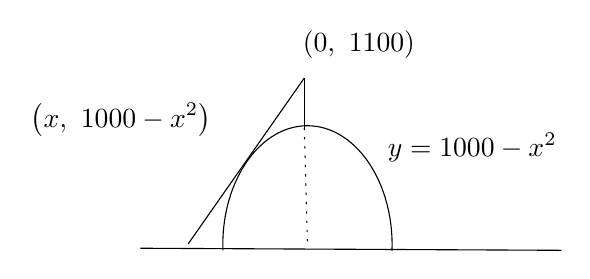
\begin{tikzpicture}[x=0.75pt,y=0.75pt,yscale=-1,xscale=1]
%uncomment if require: \path (0,300); %set diagram left start at 0, and has height of 300

%Straight Lines [id:da5723816642656105] 
\draw    (161,231) -- (364,232) ;
%Shape: Arc [id:dp6981731539336795] 
\draw  [draw opacity=0] (200.8,232.01) .. controls (200.77,231.15) and (200.76,230.28) .. (200.75,229.4) .. controls (200.73,197.7) and (218.96,171.99) .. (241.48,171.97) .. controls (264,171.95) and (282.28,197.63) .. (282.31,229.33) .. controls (282.31,230.27) and (282.29,231.19) .. (282.26,232.12) -- (241.53,229.37) -- cycle ; \draw   (200.8,232.01) .. controls (200.77,231.15) and (200.76,230.28) .. (200.75,229.4) .. controls (200.73,197.7) and (218.96,171.99) .. (241.48,171.97) .. controls (264,171.95) and (282.28,197.63) .. (282.31,229.33) .. controls (282.31,230.27) and (282.29,231.19) .. (282.26,232.12) ;  
%Straight Lines [id:da28537975742427224] 
\draw    (240,149) -- (240,173) ;
%Straight Lines [id:da508714474634949] 
\draw    (240,149) -- (184,229) ;
%Straight Lines [id:da9548957625218735] 
\draw  [dash pattern={on 0.84pt off 2.51pt}]  (240,173) -- (241.53,229.37) ;

% Text Node
\draw (279,174) node [anchor=north west][inner sep=0.75pt]   [align=left] {$\displaystyle y=1000-x^{2}$};
% Text Node
\draw (238,125) node [anchor=north west][inner sep=0.75pt]   [align=left] {$\displaystyle ( 0,\ 1100)$};
% Text Node
\draw (107,160) node [anchor=north west][inner sep=0.75pt]   [align=left] {$\displaystyle \left( x,\ 1000-x^{2}\right)$};
\end{tikzpicture}
\\
\\
The slope at point $x$ on the graph is $\frac{dy}{dx} = -2x$. At the same time the slope of the line that goes through the points $(x, 1000-x^2$ and $(0, 1000)$ is $\frac{1100-(1000-x^2)}{0-x}$. So we have to solve an equation for $x$.

\[
\frac{1100-(1000-x^2)}{0-x} = -2x
\]
\[
100+x^2 = 2x^2
\]
\[
x^2 = 100
\]

 The ant begins to see the tower at height $y = 1000-100 = 900$.

\subsection{Problem 4}
\begin{itemize}
 \item[(a)] $y = \frac{x^2}{4p}$, the slope at point $x$ is equal to $\frac{dy}{dx} = \frac{x}{2p}$.
 The tangent line has form $y = \frac{dy}{dx}x + b$. The $y$-intercept is equal to $b$ when $x = 0$. So at point $(x_0, y_0)$ we have an equation:
 \[ y_0 = \frac{x_0}{2p}x_0 + b \]
 \[ b = y0 - \frac{x_0^2}{2p} \]
 \[ \frac{x_0^2}{2p} = 2y_0 \]
 \[ b = y_0 - 2y_0 = -y_0 \]

\item[(b)] Let $A = (0,p)$, $B = (x_0, y_0)$ and $C = (0, -y_0)$.\\
\\
The distance formula $D = \sqrt{(x_2 - x_1)^2 + (y_2 - y_1)^2}$. 
\\ \\
$D_{AB} = \sqrt{x_0^2 + (y_0-p)^2} = \sqrt{x_0^2 + y_0^2 - 2y_0p + p^2} = \sqrt{x_0^2+\frac{x_0^4}{16p^2}-\frac{2x_0^2p}{4p}+p^2} =$ \\ \\ $\sqrt{\frac{16x_0^2p^2+x^4-8x_0^2p^2+16p^4}{16p^2}} = \sqrt{\frac{x_0^4+8x_0^2p^2+16p^4}{16p^2}} = \sqrt{\frac{(x_0^2+4p^2)^2} {16p^2}}=\frac{x_0^2+4p^2}{4p} = $ \\ \\ $\frac{x_0^2}{4p}+p$ \\ \\ \\ \\
$D_{AC} = \sqrt{(-y_0-p)^2} = \sqrt{y_0^2 + 2y_0p + p^2} = \sqrt{\frac{x_0^4}{16p^2} + \frac{2x_0^2p}{4p} + p^2} = $
\\ \\
$\sqrt{\frac{x_0^4+8x_0^2p^2+16p^4}{16p^2}} = \sqrt{\frac{(x_0^2+4p^2)^2}{16p^2}} = \frac{x_0^2+4p^2}{4p} = \frac{x_0^2}{4p} + p$ \\ \\

The triangle is isosceles as $D_{AB} = D_{AC}$.
\item[c)]
Let's take reflection point $B$. Without loss of generality we show that ray $BE$ is parallel to the axis. As shown in $(b)$ the triangle $ABC$ is isosceles. The base of triangle is $BC$ and angles $\alpha$ and $\beta$ are equal. Since angles $\alpha$ and $\theta$ are equal by definition, it implies that $\beta = \theta$. Ray $CA$ is parallel to the axis as shown in the picture. That implies that ray $BE$ is also parallel to the axis. 
\begin{figure}[htp!]
    \centering
    \includesvg{diagram-1.svg}
    \label{fig:fig3}
\end{figure}
\end{itemize}

\subsection{Problem 5}
\begin{itemize}
\item[a)] 
$V = \frac{(10-t)^2}{5}$ \\ \\ 
$\frac{\Delta V}{\Delta t} = \frac{V(0) - V(5)}{0 - 5} = \frac{20 - 5}{-5} = -3\; l/m$.

\item[b)]
$\frac{dV}{dt} = -\frac{2}{5}(10-t)$ \\ \\
When $t = 5$, then $\frac{dV}{dt} = -2\; l/m$

\subsection{Problem 6}

\begin{itemize}
\item[(19d)] 
\[\lim_{x\to \infty}x\sin\ \frac{1}{x}\]
\[x = \frac{1}{u}\]
\[\lim_{u\to 0}\frac{\sin u}{u} = 1\]

\item[(19f)]
\[\lim_{x \to 0}\frac{\sin^2 x}{3x^2} = \lim_{x \to 0}\left[ \frac{1}{3}\frac{\sin x}{x}\frac{\sin x}{x} \right] = \frac{1}{3}\]

\item[(19g)]
\[ \lim_{x \to 0} \frac{\sin 2x}{\sin 3x}  \]
\[ \frac{\sin 2x}{\sin 3x} = \frac{2 \sin x \cos x}{\sin (x + 2x)} = \frac{2 \sin x \cos x}{\sin x \cos 2x + \cos x \sin 2x} \]
\[ = \frac{2 \sin x \cos x}{\sin x \cos 2x + \cos x (2 \sin x \cos x)} \]
\[ = \frac{2 \cos x}{\cos 2x + 2 \cos^2 x} \]
\\
\[ \lim_{x \to 0} \frac{2 \cos x}{\cos 2x + 2 \cos^2 x} = \frac{2}{3}\]

\item[(20c)]
\[ \lim_{x \to 0} \frac{x^2}{1 - \cos^2 x} =  \lim_{x \to 0} \frac{x^2}{\sin^2 x} = 1\]

\item[(20g)]
\[
\lim_{x \to 0} \frac{3x^2+4x}{\sin 2x} = \lim_{x \to 0} \frac{x(3x+4)}{2 \sin x \cos x} = \lim_{x \to 0} \frac{x}{2 \sin x} \cdot \frac{3x + 4}{\cos x} = \frac{1}{2} \cdot 4 = 2
\]

\item[(22a)]
\[
L = \lim_{\theta \to 0} \frac{1 - \cos \theta}{\theta^2}
\]
\begin{itemize}
    \item[(a)]
    \begin{tabular}{|c|c|}
    \hline
     $\theta$ & $L$ \\
    \hline
    $0.1$ & $0.49958$ \\
    $0.01$ & $0.49999$ \\
    $0.001$ & $0.49999$ \\
    $0.0001$ & $0.49999$ \\
    \hline
    \end{tabular}
    \\ \\
    We see from the results of calculations that $L = \frac{1}{2}$.

    \item[(b)]
\[ \lim_{\theta \to 0} \frac{1 - \cos \theta}{\theta^2} = \lim_{\theta \to 0} \left(\frac{1 - \cos \theta}{\theta^2} \cdot \frac{1 + \cos \theta}{1 + \cos \theta} \right)\]
\[ = \lim_{\theta \to 0} \frac{1 - \cos^2 \theta}{\theta^2(1 + \cos \theta)} = \lim_{\theta \to 0} \frac{\sin^2 \theta}{\theta^2(1 + \cos \theta)}\]
\[ = \lim_{\theta \to 0} \left( \frac{\sin^2 \theta}{\theta^2} \cdot \frac{1}{1 + \cos \theta} \right) \]
\[ = 1 \cdot \frac{1}{1 + 1} = \frac{1}{2}\]
    
\end{itemize}

\end{itemize}

\subsection{Problem 7}
\begin{itemize}
\item[a)] 
$D(uvw) = (uv)'w + uvw' = (u'v + uv')w + uvw' = u'vw + uv'w + uvw'$
\item[b)]
$D(u_1u_2 \dots\ u_n) = u_1'u_2 \dots un + u_1u_2' \dots u_n + u_1u_2 \dots u_n'$ \\ \\
Let's prove that statement by induction. The base case is presented in $(a)$. Suppose that the guessed formula for $D(u_1u_2 \dots\ u_n)$ is true. We need to show that it's also true for $D(u_1u_2 \dots\ u_nu_{n+1})$. \\
Let $w = u_1u_2 \dots\ u_n$. \\
Now $D(wu_{n+1}) = w'u_{n+1} + wu_{n+1}' = (u_1'u_2 \dots un + u_1u_2' \dots u_n + u_1u_2 \dots u_n')u_{n+1} + (u_1u_2 \dots\ u_n)u_{n+1}' = u_1'u_2 \dots unu_{n+1} + u_1u_2' \dots u_nu_{n+1} + u_1u_2 \dots u_n'u_{n+1} + u_1u_2 \dots\ u_nu_{n+1}'$.
\end{itemize}

\end{itemize}

\end{document}
